
\documentclass[manuscript,screen,review]{acmart}
\settopmatter{printacmref=false}
\AtBeginDocument{%
  \providecommand\BibTeX{{%
    Bib\TeX}}}


\begin{document}

\title{Exploration of orchestration challenges in a microservice-based application}


\author{Luca Marchiori}
\email{luca.marchiori.3@studenti.unipd.it}
\affiliation{%
  \institution{Runtimes for Concurrency and Distribution 2023-2024 - University of Padua}
  \country{Italy}
}

\begin{abstract}
  The following is a technical report related to the course, "Runtimes for Concurrency and Distribution," conducted by Prof. Tullio Vardanega at the University of Padua. This report aims to summarize what was learned when approaching the concepts of microservices and orchestrations, and highlight the discoveries made by implementing a proof of concept practical example.
\end{abstract}

\maketitle


\section{Problem statement}
The selection of this project, among others, was driven by the desire to dedicate time to exploring the microservices architecture. Microservices, like many other paradigms in the past, appear to be the (almost) new and shiny approach that developers seek to adopt. However, determining whether the microservices architecture is a good fit for a specific problem is a completely different matter and requires a good understanding of both technologies involved and the concepts behind the architecture.

Starting from the definition of microservices and reviewing the course material, I have adopted an exploratory approach to understand different areas of this architecture. I began by implementing virtualization and containerization, and then moved on to the concepts of  container orchestration, service state management, and finally, communication between services implementing both synchronous and asynchronous communication styles.

\section{Scope and purpose}
After reviewing numerous resources, both online and in books, my focus has been centered on three different aspects that are included in every definition of microservices. These aspects are: independent deployability, communications strategies and business domain logic. 

Each aspect covers multiple concepts. When exploring how microservices can be independently deployed, the principles of encapsulation, information hiding, and state management have been at the core of my experiments.

Communication plays a crucial role in defining how microservices can interact with each other and how this impacts the final responsiveness of the systems. This includes both the style of communication (synchronous, asynchronous) and the technology used (HTTP, RPC, etc.).

The selection of a business domain for a microservice is more conceptual than technological. It requires a holistic view of the entire architecture and precise planning to ensure that no business domain is shared or redundant. It is also necessary to ensure that each microservice can effectively address the needs of the domain it is designed for.

The recurring concept of scalability covers all of these three aspects, starting from the technological choices, up to how microservices can be managed effectively by multiple teams and make the development also scaling with the company. More on this in the following sections.

\section{Experimental implementation}
During the exploration of these concepts and related technologies and tools, some basic components of a potential architecture have been developed as experimental examples. The aim was to implement components commonly found in any software, such as user management and authentication.


\subsection{Containerization}
The project has begun with the study of Docker, one of the most famous containerization platforms available today. Containerized microservices are crucial for ensuring the microservice's independence from the underlying infrastructure and for facilitating easy deployment. This is achieved by encapsulating everything needed to run the software logic into a single object, ranging from a minimal version of an operating system to runtimes, libraries, and storage volumes.

With containers, it is possible to create multiple execution environments that are completely isolated from each other, without the overhead of a hypervisor. This is achieved by leveraging a single kernel shared between containers and abstracting the processes of the individual virtualized environments. With tools such as Docker Swarm and Kubernetes, managing hundreds of containers running on different physical servers becomes possible. Indeed, containerization is at the base of the independent deployability property of microservices.

For the practical implementation, a small web service has been created that provides a handler to accept HTTP POST requests to create a user profile with the provided information. After this, a completely containerized version of this web service was developed.

The first thing I created was a DockerFile with a multi-stage build process. This type of DockerFile allowed me to containerize the compilation of the microservice, making it completely self-contained. The first stage, responsible for the actual build, uses a base image optimized to include all the necessary GO tools for the compilation of GO software. After downloading all the dependencies and required libraries, the actual build process begins. In the end, the binary is transferred to a more essential base image that uses Alpine Linux as its OS and simply runs the already created executable file. The multi-stage feature allowed me to compile the service in a heavier environment with all the necessary tools for compilation, and then transfer the binary to a minimal image that can be moved and deployed with minimal resources. Since the web service is set to provide service on port 4000, a declaration in the DockerFile is included to expose that port.

The created image needs to be loaded into an image registry to make it available to other deployment systems like Kubernetes. A container registry is a repository (or collection of repositories) used to store and access container images. These can be hosted locally or on a cloud provider and provide storage to have all the images in one place that can be pulled by other software. The registry also provides version control to catalog all the different versions of a piece of software and multiple security mechanisms to ensure that only authorized entities can access the images. Since cloud providers that offer image registries often require payment, I chose the Google Cloud Artifact Registry that has a free plan for testing purposes.

The process of configuring Docker to interact with Google Cloud has been quite difficult due to the numerous security policies needed to ensure authentication to the system and authorization of operations. After reading some documentation and installing the required packages by Google to enable some Docker configurations, I was able to push and pull images from Google Cloud Artifact Registry.

Since the application also needs a database connection to store and retrieve users, a new container built with a PostgreSQL DB image has been created. Thanks to a Docker Compose file, it's possible to configure the container of the application logic and the container with the database instance to communicate and run together. Of course, the database image needs to have a persistent state in order to keep the data across restarts. This is a problem that I have encountered many times during the project implementation, and I will focus on it in the next sections. For now, the solution is simply to map a folder on the host machine to the one that the containerized database uses to store data, thanks to the configuration of volumes in the docker-compose file.

\subsection{Container limitations}
The solution developed so far has been working well and has had no issues handling the requests made by me and some tools such as curl and Swagger \footnote{Swagger is an open-source framework for designing, building, documenting, and consuming RESTful web services.}. In fact, many softwares are deployed in this way and are perfectly suitable for non-critical operations, test environments, or very controlled production environments with few users. However, it would be careless to adopt the same deployment strategy for a critical, high availability service that needs to be operational 24/7 with a large user base. Here are some of the most evident limitations:

\textbf{Scalability}: One of the limitations is the inability to scale the container dynamically. Since it is hosted on a single server, it cannot be replicated or have its resources scaled up to accommodate higher demand. The only option would be to manually move it to a more powerful server or upgrade the server itself. However, this process cannot be done dynamically to optimize resources and service costs depending on the real demand. Additionally, during the upgrade, there is a risk of downtime and potential compromise of the system’s availability.

\textbf{Updates}: In order to update the microservice, the container needs to be stopped, updated, and then started again. The issue here is not only the downtime but also the lack of available strategies in case the update encounters problems. Until the developer realizes that the update is faulty, users may have access to a flawed version of the software, which could potentially be dangerous for the whole system. Ideally, we would like to have updates that can be performed without any downtime, and have strategies to detect errors and rollback to the previous version without users being aware of it.

\textbf{Errors}: Although it is possible to define the behavior of a container in the event of a software crash (by setting the restart property), it can be challenging to define custom mechanisms to handle container failures. Additionally, the definition of failure itself requires careful attention, as we would want to restart the service not only in the event of a software crash but also in cases of unresponsiveness, custom errors, or timeouts. Furthermore, the restarting of a single container also takes time, during which the service would be unavailable.

\textbf{Networking}: When dealing with multiple microservices that need to be connected and exchange data, Docker provides limited control over networking by using only a virtualized internal network. Manually defining network links and addresses can be challenging, and failures can occur due to the dynamic nature of web services that may change IP addresses or be moved across servers. Additionally, we would want to define links that are accessible to users for accessing the services, while keeping internal links hidden from the public and used only for internal communications.

\textbf{Deployment}: The manual installation and management of Docker containers on specific nodes can be hard and require constant effort to ensure they stay online and error-free. Ideally, we would prefer to have a centralized method for managing the deployment of services across multiple nodes. This would simplify the process and make it easier to maintain and monitor the containers effectively.

Those are all desirable features that can only be achieved by using orchestration software, which provides automated deployment, coordination, and management of services. It's important to note that orchestration is not limited to microservices alone, it is a broader concept that can be applied to a wide range of distributed systems and application architectures. In the context of microservices, orchestration plays a crucial role, but it can also be used in other types of systems. One of the most well-known orchestration platforms is Kubernetes.

After realizing the many limitations related to orchestration of the simple solution developed so far, I have decided to start working with Kubernetes. I have configured a local cluster with the installation of Minikube \footnote{\href{https://minikube.sigs.k8s.io/docs/}{Minikube} is a tool that allows to run a KUbernetes cluster in a virtualized and local enviroment.} and have begun working on configuring the various objects required to run the software architecture.

\begin{figure}[h]
  \centering
  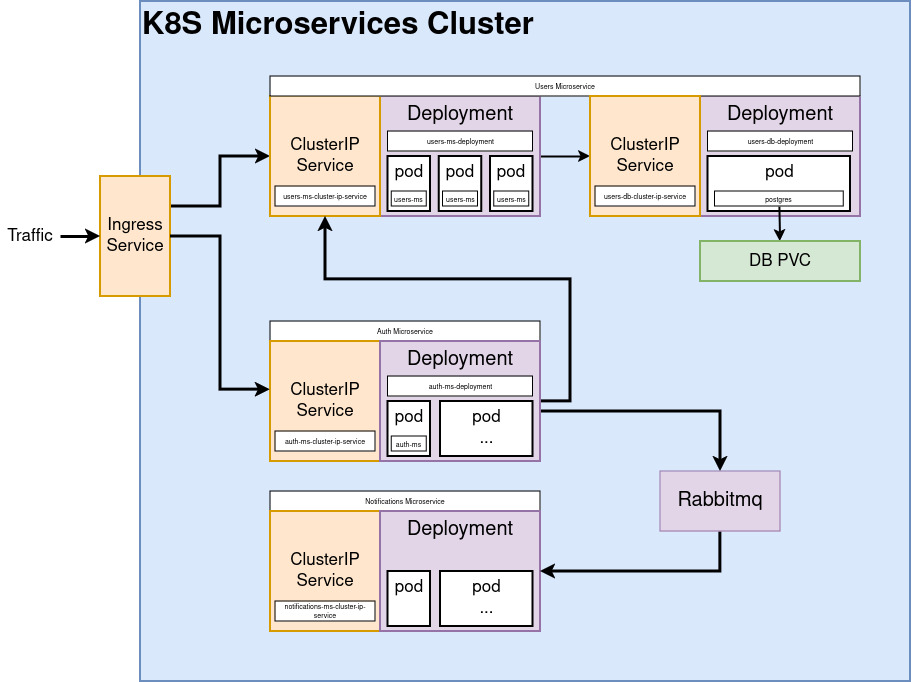
\includegraphics[width=0.5\textwidth]{Images/Cluster.jpg}
  \caption{Architecture of Kubernetes cluster for the practical implementation}
\end{figure}


\subsection{Users Microservice}
The Users Microservice defines different handlers for the management of a user base. All the handlers use HTTP and the REST (Representational State Transfer) paradigm and are exposed on port 4000.

\begin{itemize}
    \item POST: /users-ms/users receive a json containing name, surname, email and other user information to store in the database.
    \item GET: /users-ms/users/{id} receive an integer that is used to retrieve the user with the corresponding id.
    \item GET: /users-ms/users return the list of all users. Additional parameters such as email, name, surname, can be passed to filter out the results.
    \item PUT: /users/{id} retrieves a user with the corresponding id passed as parameter and updates its information with the data provided.
    \item DELETE: /users/{id} simply deletes a user with the corresponding id.
\end{itemize}

An architectural decision needs to be made to determine how the internal state of the microservice is managed. This state must be persistent to ensure that the stored user information persists across multiple requests and service restarts. A common solution to this issue is to use a database.
As stated before, microservices should be self-contained and hide their internal state so that any mechanism to manage the internal state is considered to be hidden inside the microservice itself. At the same time we would want to have microservices independently deployable and to be able to implement horizontal scaling through replication. This leads to the possibility of having multiple instances of the same microservice running at the same time.

Having multiple instances of a service allows it to handle more traffic and improve the reliability of the microservice as it can easily tolerate the failure of a single instance, restart it and divert the traffic to other instances at the same time.

In this case, the assumption of having one database included in each instance is completely wrong and can lead to distrasours outcomes in terms of state (and data) integrity. A desirable way to cope with this situation is to have the database in a single instance accessible only by all the instances of the microservice related to the database. More on this on the next subsection.

The basic configuration of Kubernetes (a.k.a K8s) for the users microservice involves the creation of a yaml file that defines three different objects: a development, a node port service and a cluster ip service. The deployment object is in charge of pulling the image from google cloud and deploying multiple pods depending on the specific configuration. The node port service maps the port 4000 of a pod to the port 30400 of the host. This configuration allowed me to directly access the service for testing and debugging purposes without having to pass through the cluster ip service. The cluster ip service assigns the port 4000 to the deployment in order for the microservice to be accessed internally by other objects of the cluster.

Since pods can be created, deleted and restarted both as a mechanism to recover from failures and as a way of dealing with updates and scaling, the ip addresses of the pods associated with a deployment change continuously. Configuring a cluster using fixed ip addresses would simply not be feasible and indeed is a big problem when dealing with orchestration of services. To solve this problem, kubernetes services use selectors to bind to other objects identified by labels. An internal DNS mechanism allows translating the binding between labels and selectors to actual ip addresses. Thanks to this the routing of connections between pods and nodes hosted on different servers can be abstracted and configured simply by using labels. This mechanism is often referred to as “Service Discovery” and it is a key feature that allows for effective orchestration by solving many problems related to networking.

\subsection{Users DB Microservice}
This microservice is used by the users microservice to maintain a persistent state of the users' information. The deployment object retrieves a PostgreSQL image directly from the official image registry (in this case, Docker Hub) and configures the database using environment variables for the name, user, and password required for access. To ensure that there is only one instance of the database running at any time, the replicas parameter is set to 1.

As before, the node port service enables direct connection to the database pod for development purposes, while the cluster IP service allows connections to the database from other nodes in the cluster. Only the user's microservice is configured with the appropriate environment variables to access the database. Thanks to the service discovery mechanism, there is no need to manually configure deployments with specific IP addresses.
The database deployment is identified by the "users-db" label. Through the cluster IP service and service discovery mechanism, the users microservice accesses the database by connecting to the endpoint "users-db-cluster-ip-service".

To allow persistence across service restarts, a PersistentVolume object is connected to the deployment through a pre-defined PersistentVolumeClaim. The ReadWriteOncePod policy is implemented to allow the volume to be mounted as read-write by a single node and a single pod, specifically the instance running the users database.

It is evident that using a DB instance of this kind has no way of scaling horizontally and can only be upgraded by assigning more resources to it. However, the microservice architecture itself helps with the scalability of the database because the state of the whole system is already split into many different databases that can better handle the traffic. Anyway, there is still the possibility of having a microservice so important that the database linked to it needs a better way to scale.

The first solution is to delegate the management of the database to a third-party service, like a cloud provider, that is responsible for scaling the database depending on the traffic and the service's requirements. This may introduce an additional cost to the system, but it can make it easier for small development teams to scale the service. 
The second option is to implement a distributed database that can be managed by Kubernetes itself or other systems.
By researching documentation, I discovered that Zalando, the well-known online shop, has deployed a Postgres Operator for Kubernetes that supports functionalities such as load balancing, cluster deployments, rolling updates for the database schema, point-in-time recovery, and many others. The operator is completely open source and available for implementation.
I haven't implemented this feature because it would have required more focus on it rather than on the main goal of the project. However, it is an interesting option that may be worth exploring.

\subsection{Auth Microservice}
To test the communication between two microservices, the Auth Microservice has been created. This service has just one handler (POST: /auth-ms/auth/login) that receives a username and a password and returns a token if the credentials match a user registered in the system. The underlying idea was to implement a simple example of a standard authentication system that operates through tokens. These systems work by generating a token to identify and authorize subsequent requests after a user has been authenticated using credentials.

In this version, the auth microservice sends a GET request to the users microservices providing the email of a user. If found, the users microservice returns the user, and the auth microservice checks if the provided password matches the one associated with the user. If so, a random token is generated and returned as a response.

The connection between the two services is managed by the internal service discovery mechanism, and the configuration does not involve the management of actual IP addresses but only the use of labels.

As a security measure, passwords should never be stored in plain text or transmitted over insecure connections. In my implementation, the password is hashed using bcrypt, one of the safest password hashing tools, as soon as it is received by the microservice. The comparison between the stored password and the one provided is also done using a bcrypt function. Note that to maintain the separation of business domains in microservices, the auth service does not directly access the database, instead, it requests user retrieval from the users service. This way, each microservice is responsible for managing its functions, and all the underlying work is hidden and managed by the microservice itself.

The GET request to the users microservice is synchronous and blocking: the auth microservice cannot proceed until it receives a response. Although synchronous connections may have limitations in terms of system responsiveness, in this case, it is needed since user retrieval is a critical operation for authentication, and nothing can proceed until it is successfully completed.

To explore an asynchronous communication technique, specifically event-based, I decided that for a system like this, it would be interesting to send a notification to the user whenever a new login is triggered. Here, asynchronous communication is suitable since we do not need to wait for the notification to be sent: we can trigger the event and let another part of the system handle it. Using the RabbitMQ library, whenever a login occurs, a new message is sent to an exchange using the mailbox style of communication. The notification microservice is responsible for processing the message queues and sending the notifications.

\subsection{Asynchronous communication}
With asynchronous messaging, the microservice initiating a request can continue processing without waiting for a response while the request is transmitted over the network. In this project, event-driven asynchronous communication is used to enable the delivery of notifications upon user login. Since the sending of email can take some time, this approach allows the microservice to handle other tasks concurrently without being blocked by the request.
In the microservice architecture, one of the goals is to minimize the coupling between components as much as possible. Asynchronous communication helps us avoid temporal coupling between the authentication and notification microservices. Temporal coupling occurs when one microservice relies on another microservice to perform a specific action at the same time in order to complete an operation. By using asynchronous communication, we can decouple these services and eliminate the need for synchronous coordination, reducing dependencies and improving overall system flexibility and scalability.
In this project, RabbitMQ is used as the message broker to implement event-driven asynchronous communication. RabbitMQ is installed within the Kubernetes cluster as a cluster operator, extending the cluster's capabilities to manage the message broker automatically.
Inside the auth microservice, whenever a login event occurs, a message containing the login information is sent to an exchange that can further forward the message to different queues depending on some criteria such as routing or topics. In this case, the exchange is identified by the name “user\_login\_event” and the chosen routing strategy is “fanout”, meaning that the message is forwarder to all the queues binded to the exchange. The exchange is also set to “durable” such that it is automatically recreated in case of a restart. 
The definition of queues is on the consumer side, specifically in the Notification microservice. 
Since we would want to handle multiple type of notification both in terms of the type of event and the kind of message, i have defined the following strategy to implements queue and exchanges: the exchange is named to indicate the type of event triggered (e.g. user\_login\_event, new\_user\_event, etc.), and the queues are named after the kind of message to send (e.g. login\_email\_notification, login\_sms\_notification, etc). With this naming scheme we are free to define in a standardized way how to handle each single event of the system.

\begin{figure}[h]
  \centering
  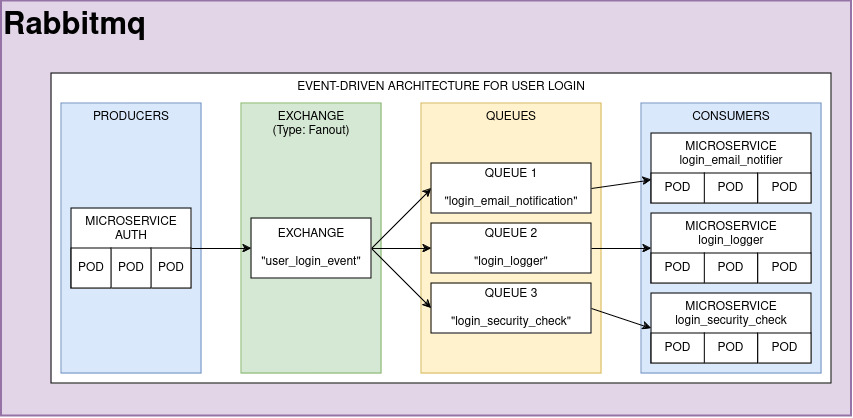
\includegraphics[width=0.8\textwidth]{Images/RabbitMQ.jpg}
  \caption{RabbitMQ scheme with producer, exchanges, queues and consumers.}
\end{figure}

\subsection{Notification Microservice}
This microservice is responsible for handling login events and sending emails to users to notify them of a new access. Upon startup, the microservice connects to the RabbitMQ instance and opens a channel on the "user\_login\_event" exchange. It then defines a non-exclusive queue named "user\_login\_event" and binds it to the exchange. The non-exclusiveness allows multiple instances of the microservice to process the queue in parallel.
Once launched, the microservice begins consuming messages from the queue, one at a time, and simulates the process of sending an email by initiating a sleep countdown. Manual acknowledgments are used to mark a message in the queue as processed only after the email has actually been sent (countdown reaches zero).
Multiple instances of the microservice are launched simultaneously, with each instance acting as a consumer. All consumers have parallel access to the queue for processing and horizontal scaling can be effectively used to elaborate the queue in parallel.

\subsection{Updates strategies}
Kubernetes allows to automate the updates of images by simply changing the desired image version in the deployment configuration. If the strategy field is not specified in the deployment configuration, the rolling update strategy is used with default values for maxSurge and maxUnavailable set to 25\% of the desired number of Pods. During the update, Kubernetes gradually replaces old Pods with new ones. The maxUnavailable field specifies the maximum number of Pods that can be unavailable during the update. For example, if the deployment has 4 replicas and a maxUnavailable of 25\%, only 1 Pod can be unavailable at any given time (or during the entire update process). The maxSurge field specifies the maximum number of Pods that can be created above the desired number of Pods. For example, if the deployment has 4 replicas and a maxSurge of 25\%, up to 1 additional Pod (for a total of 5 pods) can be created during the update process. It is also possible to use absolute numbers instead of percentages. Depending on the values of maxSurge and maxUnavailable, the update process can be faster or slower. 

In the project, the microservices related to Auth, Users, and Notifications use the default update strategy. However, the Users DB microservice uses the recreate strategy because it is not possible to have multiple instances of the same database running (maxReplicas = 1). With this strategy, when an update is triggered, the database instance is killed and replaced with the new version.

Other updates strategies are available but not implemented in the project: Blue-Green deployment and canary deployment are one of those. 

Using the latest tag for Docker images in Kubernetes environments is generally discouraged due to issues with stability, predictability, and control. The latest tag lacks clear version control, making it difficult to track and roll back versions, and can lead to inconsistent deployments since the tag can point to different images over time. This unpredictability complicates debugging and reproducing environments across development, testing, and production stages.

\subsection{Health checks}
In the first section, I highlighted that one of the challenges of orchestration is being able to detect crashes and malfunctioning components in order to restart them or take other actions to limit failures. Kubernetes allows us to define custom health checks probes to understand if a service is working properly or if there are any problems present.
The liveness probe is a configuration used to allow K8s to determine if the pod is healthy and running. The control plane checks if the applications running inside the pod containers are in some error state, and if so, it kills the container and tries to restart it. The probe can be configured to send requests (GET, POST, etc.) to a specific endpoint of the application running inside the container. If the application does not respond to the probe, the container is killed and restarted. Additional configuration parameters include the initial delay before the probe starts and the period between probes to handle custom behavior. Other types of probes, such as the readiness probe can be used to configure more advanced healthchecks.

In the practical implementation, I have defined a liveness probe on the users microservice that makes a GET request to the "/users-ms/healthcheck" endpoint every 5 seconds. Additionally, an initial delay of 5 seconds is configured for the probe to allow the microservice enough time to connect to the database upon launch. Without this delay, while the microservice is establishing internal connections and configurations, it may not respond to the health check, causing Kubernetes to mark the pod as being in an error state.

\subsection{Documentation and examples}
During the implementation, I had the need to keep track of all the endpoints of each microservice, along with the required request parameters and possible response outputs. The issue of having well written documentation is crucial for both small teams and larger companies and it is even more important in microservices architectures where there could be thousands of endpoints to manage. To address this, I decided to create an OpenAPI specification file. OpenAPI is in fact a standard specification for building APIs, providing a standardized way to describe their structure using a YAML syntax. These OpenAPI specification files can be utilized in programs like Swagger to create an environment for testing APIs. To test this out, I set up a Swagger Docker Container to access the Swagger dashboard and interact with all the endpoints.

Ideally, each microservice should have its own OpenAPI specification. This ensures that developers working on other microservices are aware of what needs to be provided to the service and what responses to expect.

\section{Experiments}
During development, in addition to verifying that the various microservices worked as intended, I did some experiments to check the actual behavior of different k8s objects.

To test the scenario of having multiple instances of the notification microservice as consumers of the RabbitMQ queue, I ran a series of consecutive login attempts on the authentication microservice. By monitoring and logging the messages received by each consumer, I was able to see that the queue was equally split between the multiple consumers, with each message being processed by only one consumer. This showed that deploying multiple concurrent and parallel consumers is an effective way of scale up message processing in a queue.

To verify the correct implementation of the liveness probe applied to the users microservice, I logged the requests made to the different pods and observed that requests were actually being sent to the microservice every 5 seconds. By intentionally causing a random crash on the microservice, I was able to see the liveness probe waiting for a response and then restarting the service.

To test the progressive update strategy, I changed the Kubernetes configuration of one microservice to use a newer image. Using the tools provided by the Minikube dashboard, I observed the different instances of the microservice stopping and updating progressively to follow the incremental update configuration.

To experiment with the Horizontal AutoScale feature of Kubernetes, I began monitoring the active replicas of the deployment both from the command line (using “kubectl get hpa users-ms-deployment --watch”) and from the Minikube dashboard. Following the suggestions from the Kubernetes documentation, I started a new pod with a simple Alpine image that continuously makes curl \footnote{cURL is a command-line tool and library for transferring data with URLs, supporting a wide range of protocols including HTTP, FTP, and many others.} requests to an endpoint of the microservice.

The load-test endpoint is designed to calculate a Fibonacci sequence to increase the CPU load. While it is true that the Fibonacci sequence is not directly related to a user management microservice, I attempted this approach because I did not observe the microservice scaling up when making requests to standard endpoints so i wanted to try with something more demanding than a simple database fetch.

However, by checking the running replicas, I did not saw the autoscaler creating new instances. My assumption is that the autoscaler may be struggling with the virtualized environment created by Minikube and is unable to accurately detect the resource usage. This assumption was further supported by the fact that the dashboard displayed CPU usage values below 0.1\%. It would be interesting to try this out in a real distributed cluster.

\section{Self-assessment}
\subsection{Project critique}
At the beginning of the project, I struggled to find a practical example to implement because every use case seemed somewhat boring and not so interesting. So, instead of focusing on creating a very special project, I chose to implement the most basic components that can be found in every cloud software available online: user management, authentication, and notifications. This approach allowed me to avoid focusing too much on the shiny features of the project itself but more on the learning of how microservices can really work. It is true that the end result is a collection of simple toy examples, but these basic examples allowed me to try many many times different configurations and get to the point of really comprehending how the orchestration of microservice works.

\subsection{Learnings}
After completing this practical implementation, I realized that orchestrating microservices does present many challenges. I had the opportunity to reflect on some of them, such as the strategies to adopt when releasing updates, the mechanisms to provide scalability, failure handling, and service discovery. The reality is that technologies like Kubernetes abstract a lot of technical implementation and make orchestration somewhat easier compared to what would be needed to do manually or how many things should be implemented to automate the process.

Even though Kubernetes and Docker can sometimes be challenging to learn and use, they are much easier than dealing with the same challenges without them. The main effort in implementing these systems is learning how to use the tools properly. Once I did that, I was able to configure everything the right way without struggling too much. 

I think that what matters is not the tool itself (such as K8s), but rather the underlying concepts. Decisions such as determining which services should run on multiple instances, choosing between synchronous or asynchronous communication, and other aspects involving concurrency and parallelism require a deep understanding of how distributed systems operate. Indeed, starting to work with Kubernetes without having taken the course on runtimes for concurrency and distribution would have been quite challenging and error-prone.


A key aspect of developing microservices that I want to highlight is beyond the technological side of things: microservices require very careful planning. We must ensure that all microservices are decoupled, independent, self-contained, and related to very specific business domains. Regardless of the technology used, these decisions require experience and a global view of the system that is far more challenging to grasp than the technologies involved.

For example, in my implementation, I spent quite some time thinking about how the auth microservice should have handled user credentials, whether the verification should have occurred in the user or authentication microservice, how much information should have been exchanged between the two, and how to recover from a possible operation failure. Similar thinking was necessary to define how the notification microservice would manage events and how to design it for future expansions to support additional events and notification mediums.

I value the learning process of these aspects much more than the learning of technology itself, because while technology can change rapidly and online resources can often resolve most doubts, reasoning about architectural choices has allowed me to better understand the design aspects of distributed systems. I am sure that this knowledge is very valuable and will be definitely helpful for me in any future projects I will work on.

Another thing that I've discovered is that while working with microservices is very interesting and has many advantages, for a small team or a single-person team, it can be more stressful than helpful.

I believe this is because as the number of microservices increases, the system becomes more and more challenging to manage, to the point where a single person loses track of all the features of each microservice and of the way microservices interact.

A better fit for microservices would be in a company with many semi-independent teams that focus on one or a few microservices and communicate with other teams regarding how their microservices interact. By following this approach, developers could focus most of their time on very specific business domains, creating the best microservices possible without needing to switch back and forth between different areas of the architecture. Then, of course, with the help of well-written documentation, it would be possible to collaborate to define the final structure of the architecture.

As is often the case, it is evident that microservices and Kubernetes are not good nor bad technologies, but rather tools that can be a good or bad fit depending on the specific use case. After completing this project, I feel like I have a better understanding of these use cases and can make more informed choices about them.
\end{document}
